\documentclass[11pt,letterpaper]{article}
\usepackage[utf8]{inputenc}
\usepackage[T1]{fontenc}
\usepackage[margin=1in]{geometry}
\usepackage{amsmath,amssymb}
\usepackage{graphicx}
\usepackage{hyperref}
\usepackage{xcolor}
\usepackage{enumitem}
\usepackage{caption}

\hypersetup{colorlinks=true,linkcolor=black,urlcolor=black,citecolor=black}
\graphicspath{{../figures/}}

\title{\textbf{The Zoo Metaverse}\\\large 3D-Native Animals, AR/VR Companion App, and Floating-Island Worlds}
\author{Antje Worring \\ \textit{Founder, Zoo Labs Foundation} \\ \texttt{antje@zoo.ngo}}
\date{October 31, 2021}

\begin{document}
\maketitle

\begin{abstract}
This element paper expands the metaverse vision from the Zoo Whitepaper~\cite{zoo2021}. Each Zoo animal is a fully-3D-rendered representation of its real-world counterpart, deployable to AR, VR, and external metaverse platforms. The companion app delivers an enchanting interactive experience, and the long-term roadmap is a Zoo-native multiverse of floating islands keyed to each animal's natural habitat.
\end{abstract}

\section{3D-Native Animals}

Every animal NFT in the Zoo ecosystem ships with FBX and WebGL formats embedded in its metadata. These are not flat images. They are full 3D models designed by visual and 3D artists, with movement, articulation, and personality consistent with the species' real-world behavior.

\begin{figure}[h]
  \centering
  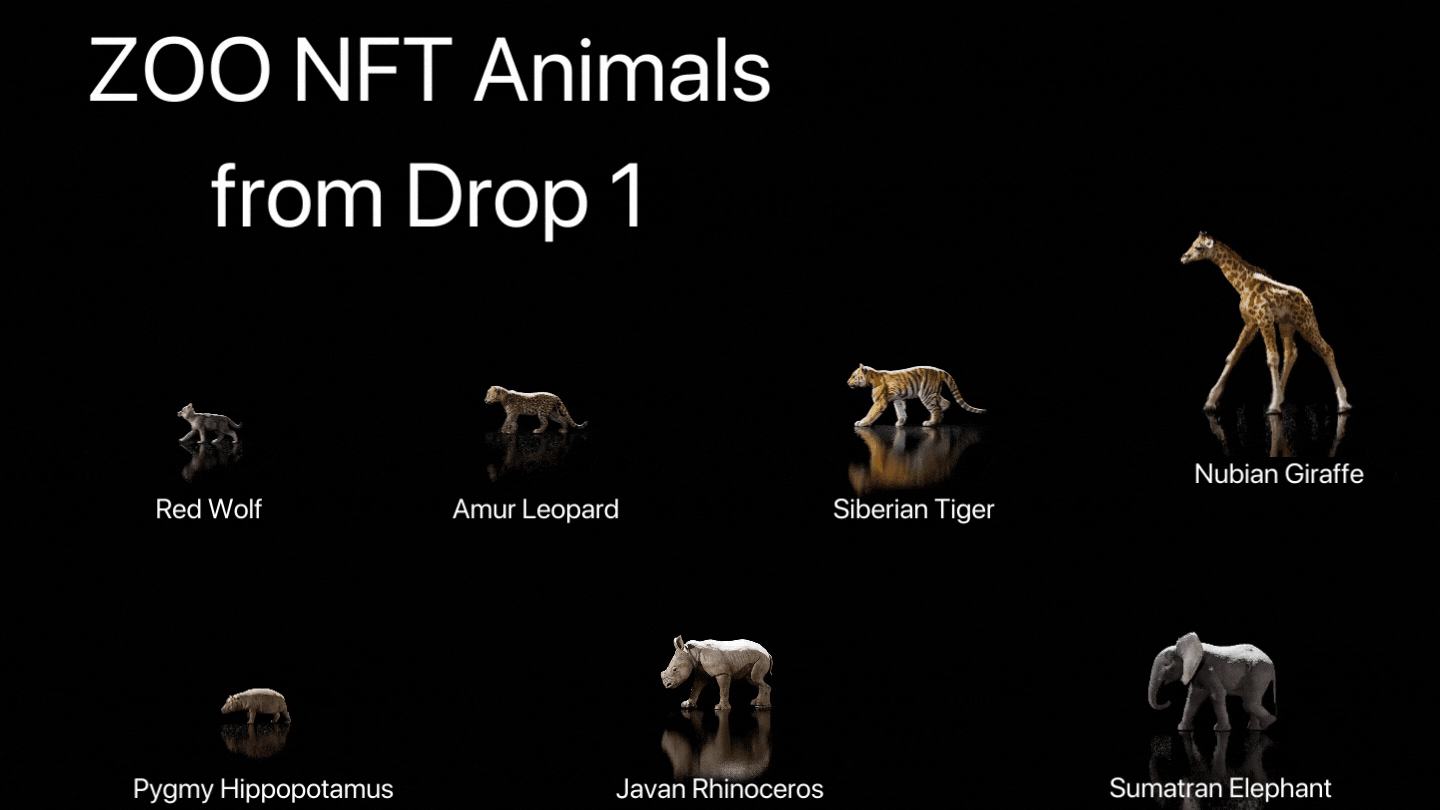
\includegraphics[width=0.85\linewidth]{animals.png}
  \caption{The Zoo metaverse companions: 3D-rendered representations of the V1 species, deployable to AR, VR, and external metaverse platforms.}
\end{figure}

\section{AR Companion App}

The Zoo iOS/Android AR companion app brings the animal into the user's physical environment. The user can place a Sublime Red Wolf on the floor of their living room and watch it pad around. The app exposes:

\begin{itemize}
  \item \textbf{Feed} --- corresponds to adding collateral on chain.
  \item \textbf{Groom and play} --- triggers idle animations and personality lines from the AI.
  \item \textbf{Share} --- snapshot to share on social media, with provenance metadata embedded.
\end{itemize}

\section{VR Experience}

In VR, the animal becomes a true companion: the user inhabits the animal's habitat, walks alongside it, and engages in quests. The whitepaper~\cite{zoo2021} describes VR as the next-level immersive surface for the Zoo experience, with mini-games and tangible rewards anchoring engagement.

\section{External Metaverse Integration}

The animal's FBX/WebGL formats let it be uploaded into any metaverse landscape. This means a Zoo Sublime Red Wolf can appear in a third-party platform's world while still being recognized on chain as the user's NFT. The whitepaper explicitly contemplates licensing and partnership opportunities with established metaverse platforms.

\section{The Floating-Island Multiverse}

The long-term roadmap describes a Zoo-native multiverse: floating islands in the cosmos, each keyed to a species' natural habitat. The Sublime Red Wolf island is a North American forest. The Amur Leopard island is a snowy Russian Far East. The Emperor Penguin island is Antarctic ice. Players can visit any island and meet the animals that inhabit it.

The multiverse is also social: users connect with friends, explore habitats together, participate in mini-games (Coin Runner, Memory Bridge), and share the joy of discovery. The intelligent avatar animals are AI-powered companions that bring the social space to life.

\section{Mini-Games and Tangible Rewards}

Two flagship mini-games launch with the metaverse:

\paragraph{Coin Runner.} The user dashes through a Zoo Labs temple, collecting gold and silver coins. Coin denominations correspond to real-world precious-metal denominations: small nuggets, larger coins, and the coveted bullion bar. Coins unlock power-ups and new animals. All rewards are redeemable for physical assets or transferable on the Zoo Market.

\paragraph{Memory Bridge.} The user crosses a treacherous bridge by memorizing a brick pattern. Failure drops the animal into lava and restarts the level. Success earns rare items, tokens, and special powers --- all redeemable for real-world rewards.

\section{Why metaverse, not just app}

The whitepaper distinguishes between an app and a metaverse. An app is a destination; a metaverse is a network. Zoo's animals are designed to be metaverse-native because the value of an emotionally intelligent companion grows with the number of contexts in which it can accompany the user. An animal that lives only inside the Zoo app is a pet; an animal that follows the user across worlds is a companion.

\section{The market context: an \$8--13 trillion opportunity}

Per~\cite{zoo2021}, leading financial institutions project the metaverse as a \$8--13 trillion opportunity by 2030 with up to 5 billion users. Zoo's positioning is not opportunistic. The intersection of conservation, AI companions, and immersive worlds is what gives Zoo a defensible niche in a market that will otherwise be dominated by general-purpose social and gaming metaverses. We are deliberately specialized: ours is the metaverse of empathy with the animal kingdom.

\section{XR continuum: AR \texorpdfstring{$\to$}{->} MR \texorpdfstring{$\to$}{->} VR}

The whitepaper uses the umbrella term \emph{XR} (extended reality) to span:

\begin{itemize}
  \item \textbf{AR (Augmented Reality)} --- animal placed into the user's physical environment via phone camera. Lowest friction, highest reach.
  \item \textbf{MR (Mixed Reality)} --- animal interacts with surfaces and lighting of the physical environment. Requires depth-sensing hardware.
  \item \textbf{VR (Virtual Reality)} --- user enters the animal's habitat. Highest immersion, requires headset.
\end{itemize}

A single Zoo animal projects onto all three modes through one identity. The whitepaper~\cite{zoo2021} explicitly emphasizes that the same companion is reachable from any of these surfaces.

\section{Tamagotchi as ancestor}

The whitepaper~\cite{zoo2021} cites Tamagotchi as the conceptual ancestor of the Zoo experience: a virtual pet that the user cares for via simple inputs. Tamagotchi was first released in 1996 by Bandai and sold over 80 million units worldwide. The simplicity of caring-for-a-creature has perennial appeal. Zoo updates this primitive for Web3:

\begin{itemize}
  \item Tamagotchi pets had no real-world value. Zoo animals do (collateral, rewards, asset-backed token).
  \item Tamagotchi pets ran on disposable hardware. Zoo animals are owned via cryptographic keys, portable across all surfaces.
  \item Tamagotchi pets had limited interaction loops. Zoo animals have AI-driven, open-ended conversation.
  \item Tamagotchi pets had no conservation impact. Zoo animals route real value to non-profit conservation partners.
\end{itemize}

\section{Seven elements most NFT games lack}

The whitepaper~\cite{zoo2021} enumerates seven elements that the broader NFT-gaming category typically fails to deliver and that Zoo provides:

\begin{enumerate}
  \item A clear path to quick and meaningful ROI through the unique staking-and-store-of-value approach.
  \item True 3D rendering with movement and personality, not flat sprite art.
  \item AR/VR/Metaverse readiness from the day of mint.
  \item AI-driven personalities that grow with the user.
  \item Conservation impact tied to every transaction.
  \item DAO-driven governance of game and protocol parameters.
  \item Open-source posture and educational pipeline.
\end{enumerate}

\begin{thebibliography}{1}
\bibitem{zoo2021} Antje Worring. \emph{Zoo: A Game-Fi Multiverse Ecosystem for the Preservation of Endangered Species}. Zoo Labs Foundation, October 31, 2021.
\end{thebibliography}

\end{document}
